% !TEX TS-program = pdflatex
% !TEX encoding = UTF-8 Unicode

% This is a simple template for a LaTeX document using the "article" class.
% See "book", "report", "letter" for other types of document.

\documentclass[11pt]{article} % use larger type; default would be 10pt

\usepackage[utf8]{inputenc} % set input encoding (not needed with XeLaTeX)

%%% Examples of Article customizations
% These packages are optional, depending whether you want the features they provide.
% See the LaTeX Companion or other references for full information.

%%% PAGE DIMENSIONS
\usepackage{geometry} % to change the page dimensions
\geometry{a4paper} % or letterpaper (US) or a5paper or....
% \geometry{margin=2in} % for example, change the margins to 2 inches all round
% \geometry{landscape} % set up the page for landscape
%   read geometry.pdf for detailed page layout information

\usepackage{graphicx} % support the \includegraphics command and options

% \usepackage[parfill]{parskip} % Activate to begin paragraphs with an empty line rather than an indent

%%% PACKAGES
\usepackage{booktabs} % for much better looking tables
\usepackage{array} % for better arrays (eg matrices) in maths
\usepackage{paralist} % very flexible & customisable lists (eg. enumerate/itemize, etc.)
\usepackage{verbatim} % adds environment for commenting out blocks of text & for better verbatim
\usepackage{subfig} % make it possible to include more than one captioned figure/table in a single float
% These packages are all incorporated in the memoir class to one degree or another...

%%% HEADERS & FOOTERS
\usepackage{fancyhdr} % This should be set AFTER setting up the page geometry
\pagestyle{fancy} % options: empty , plain , fancy
\renewcommand{\headrulewidth}{0pt} % customise the layout...
\lhead{}\chead{}\rhead{}
\lfoot{}\cfoot{\thepage}\rfoot{}

%%% SECTION TITLE APPEARANCE
\usepackage{sectsty}
\allsectionsfont{\sffamily\mdseries\upshape} % (See the fntguide.pdf for font help)
% (This matches ConTeXt defaults)

%%% ToC (table of contents) APPEARANCE
\usepackage[nottoc,notlof,notlot]{tocbibind} % Put the bibliography in the ToC
\usepackage[titles,subfigure]{tocloft} % Alter the style of the Table of Contents
\renewcommand{\cftsecfont}{\rmfamily\mdseries\upshape}
\renewcommand{\cftsecpagefont}{\rmfamily\mdseries\upshape} % No bold!

%%% END Article customizations

%%% The "real" document content comes below...

\title{CS211 Wordladder Assignment}
\author{Jacob Smith <jas32>}
%\date{} % Activate to display a given date or no date (if empty),
         % otherwise the current date is printed 

\begin{document}
\maketitle

\section{Program Invocation}

\subsection{Generation mode}
The program can be invoked in generation mode with \texttt{java -jar wordladder.jar <start word> <depth>}. This produces a random word ladder with \texttt{start word} as the first entry out to the depth specified by \texttt{depth} assuming such a word ladder is possible with the dictionary included.

\subsection{Discovery mode}
The program can be invoked in discovery mode with \texttt{java -jar wordladder.jar <start word> <end word>}. This produces a word ladder with the given start and end points. It will attempt to construct the shortest word ladder possible using the included dictionary.

\section{Class Schema}

\begin{figure}[h!]
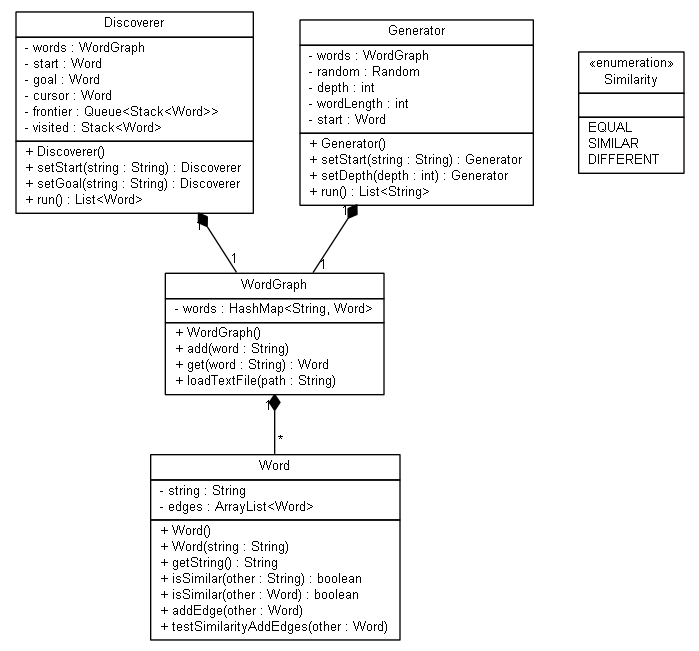
\includegraphics[width=\textwidth]{ClassDiagram}
\caption{Class Diagram for uk.ac.aber.cs211.wordladder package.}
\end{figure}

The \texttt{Word} object encapsulates a word as a part of a graph whose edges represent valid transitions to 'similar' words (ie those with exactly one different character). These edges are stored as an \texttt{LinkedList<Word>} (the many:many aggregation is not pictured). A LinkedList is used as this structure is typically very small and both Generator and Discoverer need to remove edges that are no longer promising frontiers for expansion. The method \texttt{testSimilarityAddEdges(Word)} compares a word with this one, if they are 'similar' it adds a pair of edges between them (one in each direction). It is this method which is used to populate the graph.

\texttt{WordGraph} stores the dictionary of words known to the program. It may be interrogated for a particular \texttt{Word} using the method \texttt{get(String)}. Words should be added to the dictionary first using \texttt{add(String)}, this behaves as a factory for new Word objects - populating their edges.

\texttt{Generator} and \texttt{Discoverer} are the entry-points into the package. Their setters are used to initialise them before being \texttt{run()}. Their algorithms (and thus attributes) are described in more detail in the next section.

\end{document}
